\documentclass[
	11pt,
	a4paper
]{scrartcl}

\usepackage[utf8]{inputenc}
\usepackage[ngerman]{babel}
\usepackage[T1]{fontenc}
\usepackage[a4paper]{geometry}
\usepackage{amsmath, amsfonts, amssymb}
\usepackage{color}
\usepackage{graphicx}
\usepackage[headsepline,automark]{scrlayer-scrpage}
\usepackage{blindtext}
\usepackage[hidelinks]{hyperref}
\usepackage{enumitem}\usepackage{float}
\usepackage{soul}
\usepackage[bottom]{footmisc}
\usepackage{tikz}
\usepackage{titlesec}

% -- CONFIG --
\definecolor{hft}{RGB}{204,49,37}
\setcounter{page}{0} % Do not count first page
\addto\extrasngerman{\def\figureautorefname{Abb.}}
\setlength\parindent{0pt}
\restylefloat{figure}
\titleformat{\section}{\normalfont\scshape\bfseries}{\thesection}{1.1em}{}
\titleformat{\subsection}{\normalfont\scshape\bfseries}{\thesubsection}{.11em}{}
\titleformat{\subsubsection}{\normalfont\scshape\bfseries}{\thesubsubsection}{1.1em}{}
\titlespacing*{\section}{0pt}{0.2cm}{0em}
\titlespacing*{\subsection}{0pt}{0.2cm}{0em}
\titlespacing*{\subsubsection}{0pt}{0.2cm}{0em}



% -- NEW COMMANDS --
\newcommand{\code}[1]{\texttt{\ul{#1}}}
\newcommand*\circled[1]{\tikz[baseline=(char.base)]{
            \node[shape=circle,draw,inner sep=2pt] (char) {#1};}}
            
% -- HEADER --
\pagestyle{scrheadings}
\clearpairofpagestyles
\setkomafont{pageheadfoot}{\upshape}
\ihead{KI Abschlussprojekt (Prof. Dr. Pado)}
\ofoot{Seite \pagemark}


% -- DOCUMENT --
\begin{document}

% -- TITLE PAGE --
\begin{titlepage}
	\makeatletter
  	\begin{center}   
       
\includegraphics[width=0.4\textwidth]{figures/HFT-logo-gross-Aplusheadline.jpg}
       \vspace{2cm}
       
       \textcolor{hft}{\hrule}
       \vspace{0.5cm}
       {\Huge\scshape Abschlussprojekt}
       \vspace{0.5cm}
       \textcolor{hft}{\hrule}
            
       \vspace{2cm}
       {\large Im Fach Künstliche Intelligenz bei Prof. Dr. Pado}
       \vspace{2cm}
       
       
       \begin{flushleft}\quad Aufgabenstellung:\end{flushleft}
       {\large \textbf{Newsgroups}}
       \vspace{1cm}
       
       \begin{flushleft}\quad Teilnehmer:\end{flushleft}
       {\large Jochen Spender (1000146}\\\vspace{0.1cm}
       {\large Luca Lissner (1002327)}\\\vspace{0.1cm}
       {\large Mario Podda (379210)}\\\vspace{0.1cm}
       {\large Samuel Maier (1002330)}
       \vspace{1cm}
       
       \begin{flushleft}\quad Abgabe:\end{flushleft}
       {\large 18. November 2021}
   \end{center}
\end{titlepage}

% -- TABLE OF CONTENTS AND SOURCES --
%\newgeometry{lmargin={2cm},rmargin={2cm},tmargin={2.5cm},bmargin = {2.5cm}, headsep={0.3cm}}
\newgeometry{left=2cm, right=2cm, top=1.2cm, bottom=1.2cm,includehead,includefoot, headsep=0.3cm,footskip=0.3cm,heightrounded}
\tableofcontents
\newpage

%% -- CONTENT --
\section{Dokumentation unseres Vorgehens}
Für das Präprocessing verwendeten wir Python, dieses bietet die hilfreiche NLTK Library.

Das Training wurde mit Weka durchgeführt. Wir verwendeten unterschiedliche Featurekombinationen und untersuchten auch den Nutzen einzelner Features. Die entstanden Erkenntnisse
verwendeten wir für die Entwicklung weiterer Features. Wir haben unsere Vorhaben mit \code{git} über Github synchronisiert.\\

\section{Daten}
Der \emph{20 Newsgroups} Datensatz ist eine Sammlung aus etwas 20.000 Newsgroup Beiträgen, gleichmäßig unterteilt in 20
verschiedene Themen aus den sog. Big Eight\footnote{Die \emph{Big Eight} stehen für folgende acht Bereiche: Computer,
Diskussion, Gesellschaft \& Politik, Wissenschaft, Kultur, Freizeit \& Hobby, News und Sonstiges.}. Aus einem Kommentar
aus dem Original-Datensatz geht hervor, dass der vermeintliche Autor Ken Lang die Daten für sein Projekt \emph{Newsweeder}
zusammentrug.\\
Es gibt verschiedene Versionen des Datensatzes. In unserem Datensatz wurden alle Metadaten wie Datum, Empfänger oder Betreff
entfernt, er enthält jeweils nur die tatsächliche Nachricht.\\

Für dieses Projekt erhielten wir einen Teildatensatz aus den Kategorien Raumfahrt,
Computergrafik, Religion und Atheismus. Er enthält 3370 Instanzen mit den folgenden drei Features:
\begin{enumerate}[label=\roman*), itemsep=0pt,parsep=0pt, topsep=0pt]
	\item ID: Numerisch, eine fortlaufende einzigartige Nummer über alle Instanzen
	\item text: String, enthält den entsprechenden Newsgroup Beitrag
	\item group: Nominal, die Kategorie des Textes welche unseren Zielklassen entspricht:\\
		0: Atheismus, 1: Computergrafik, 2: Raumfahrt, 3: Religion
\end{enumerate}

Wir entschieden uns, den Datensatz im Verhältnis 80:10:10 in Trainings-, Entwicklungs- und Testdaten zu trennen. Unsere Entwicklungs- und Testdaten besitzen somit jeweils 337 Instanzen, was nach AUssagender Vorlesung aureicht zur verifizierung

\section{Features}
Im folgenden eine Auflistung unserer Features. Meist wurden diese im Projektverlauf verbessert, so dass teilweise ähnliche
Versionen verfügbar sind. Auf die letztendlich benutzten Feature und ihre Nutzbarkeit wird im Abschnitt \emph{\nameref{trainingsprozess}}
näher eingegangen.

\subsection{Zeichen zählen}\label{zeichenzaehlen}
Beim Durchschauen der Texte kam uns der Gedanke, dass die Textlänge, also die Anzahl an Zeichen eines Textes, ein mögliches Feature
ist, da die Textlänge der eher technischen Texte aus den Kategorien Computergrafik und Raumfahrt oft kürzer ausfielen als die eher
philosophischen Texte aus Religion und Atheismus.\\

\subsection{Wörter zählen}\label{woerterZaehlen}
Ein weiteres Basis Feature, aus dem sich viele weitere Versionen ableiten ließen ist das zählen aus wie vielen
Wörtern ein Text besteht.\\

\subsection{Wortlänge}
Die durchschnittliche und maximale Wortlänge eines Textes könnten sich zwischen den Kategorien ändern.

\subsubsection{Wortdiversität}\label{wortdiversitaet}
Die Wortdiversität soll darstellen aus wie vielen unterschiedlichen Wörtern ein Text besteht.\\
Spezifizierend wir haben das Feature verbessert indem Stoppwörter\footnote{Unter \emph{Stoppwörtern}
versteht man sehr häufig auftretende Wörter, die meist keine direkte Relevanz für den Informationsgehalt eines Textes haben} ignoriert werden. \\

Um die Wortdiversität weiter zu verfeinern, sollten die Wörter in unterscheidlichen ausdrücken, etwa \emph{Wort} und \emph{Wörter} zusammen gezählt werden. Hierfür verwendeten wir zwei Methoden, das sog. Stemming (rein algorithmisch) und das Lemmatizing (gleicht mit Wortlisten ab).

\subsection{Bibelstellen}\label{bibelstellen}
Da Bibelstellen ein relativ einheitliches Format besitzen und sehr häufig in der Zielklasse Religion vorkommen, zählt \code{contains bible
reference number} die Anzahl an Bibelstellen pro Text.

\subsection{Wörterlisten}\label{woerterlisten}
Verschiedene Wörter kommen unterschiedlich häufig vor in verschiedenen Themenbereichen. Wir wollen das als Features abbilden.

Wir könnten manuell Wörter erfinden, aber damit müssen wir die Arbeit leisten, verpassen vermutlich Wörter, 
können weniger mit den Wörtern rumspielen, da wir nicht wirklich eine Größe dafür haben, wie relevant sie sind.

Daher bestimmen wir algorithmisch die Wörter die wir relevant finden.

\subsubsection{Präprocessing der Daten}

Zum Erstellen der Wortlisten haben wir zunächst alle Blogs Tokenized, dann die Tokenliste pro Kategorie zusammengefügt. 
Aus diesen Listen haben wir die Stoppwörter entfernt, dann den POS-Tagger angewandt und nur Nomen, Verben, Adjektive und unbekannte Wörter beibehalten.

Anschließend haben wir optional die vorhandenen Wörter gestemmt, mit nltk.PorterStemmer, oder die Wörter so belassen. 

Über das Ergebnis des ganzen haben wir die Frequenzverteilung berechnet (d.h. wie oft kommen einzelne Wörter vor). 
Diesen Schritt haben wir einmal auf den Wortlisten der einzelnen Kategorien gemacht und einmal auf auf der Kombination aller Kategorien, 
sodass wir für jedes Wort wissen, wie oft es in den einzelnen Kategorien vorkommt, und insgesamt.

Anschließend haben wir verschiedene Rankings versucht, die mit den Frequenzverteilungen erstellt wurden. 
Auf diese wird später eingegangen. Nach diesen Rankings wurden anschließend Wörter ausgesucht. 
Dabei haben wir 3 optionale Stellschrauben festgelegt: Den Ausschluss von Wörtern, 
deren Rang unter einem Schwellenwert ist und die Auswahl von N Wörtern nach Rang, einmal je nach Kategorie, einmal insgesamt.

Dann zu den Rankings. Hier wurden ein paar alternativen ausprobiert. 
Der simpelste Algorithmus verwendet einfach nur die Anzahl wie oft das Wort in seiner Kategorie vorkommt ($N_{\text{Kat, wort}}$)

Eine mögliche Verbesserung davon ist es, das Vorkommen des Wortes in der Kategorie durch das Vorkommen in allen zu Teilen ($N_{\text{Kat, wort}} / N_{\text{wort}}$). 

Dies ist allerdings Problematisch, da dadurch auch Wörter gut wegkommen, die insgesamt selten vorkommen, diese sind aber vermutlich kein guter Entscheider sondern einfach ungewöhnliche Wörter.
Daher wollen wir des weiteren die insgesamt Häufigkeit des Wortes im Vergleich zu allen Wörtern ($N_{\text{wort}} / N$) bestimmen und diese beiden Größen verknüpfen.
Eine einfache Multiplikation ($N_{\text{Kat, wort}} / N_{\text{wort}} \times N_{\text{wort}} / N$)
bewertet allerdings beide Größen ungefähr gleich. 
Dies ist eine Option, allerdings ist zu vermuten dass der neue Part weniger wichtig ist. 
Er sollte nach unserer Einschätzung nur als Größenordnung einfließen. 
Um das zu erreichen bietet sich der Logarithmus an:

\begin{equation} \label{eq-log}
	N_{\text{Kat, wort}} / N_{\text{wort}} \times log(N_{\text{wort}}) / log(N)
\end{equation}

Wir hatten noch ein paar weitergehende Ideen, wie das ein Wort höher ranken sollte wenn es in anderen Kategorien \textbf{nicht} vorkommt, 
allerdings haben unsere Versuche dies im Ranking aufzunehmen die Genauigkeit der Algorithmen lediglich verschlechtert.

\subsubsection{Erstellung von Features aus den Wörtern}

Für die ungestemmten Wörter haben wir verschiedene Wege versucht ein Feature mit den Wörtern zu erstellen:
Einmal überprüfen wir lediglich die Anwesenheit eines Wortes.
Einmal ist das Feature die relative Häufigkeit des Features in dem Blog.

Diese Features waren ein wenig teuer (in Rechenzeit) und waren, zumindest wie wir sie implementiert haben, nicht auf die gestemmten Wörter anwendbar.
Daher haben wir für diese Wörter eine andere Variante versucht, in der mit einer Regex die vorkommen gesucht wurden, 
und der Wert dadurch geteilt wurde, wie häufig das Wort in dem Blog vorkommen könnte (also die Zeichenlänge des Blogs durch die Zeichenlänge des Wortes).

\subsubsection{Ergebnisse der Vorversuche}

Bei den Rankings schlug sich zumeist die Gleichung \ref{eq-log} am besten.

In ersten Versuchen ergab die gestemmte Variante bei niedrigen Wortzahlen schnell sehr gute F-Werte, verlor allerdings bei größeren Anzahlen Genauigkeit, bis sie von der ungestemmten Variante geschlagen wurde.

\section{Trainingsprozess}\label{trainingsprozess}
Mit der Weka Funktion \emph{Visualisierung} konnten wir graphisch schnell erkennen, ob ein Feature aussagekräftig ist, wie es zum
Beispiel bei dem Wort \emph{space} für die Zielklasse Raumfahrt ist (siehe \autoref{fig:weka_visualize_space}).

\subsection{Bewertung der Features}
Der alleinige Einsatz der \emph{einfachen} Features (siehe \emph{\nameref{zeichenzaehlen}}, \emph{\nameref{woerterZaehlen}},
\emph{\nameref{wortdiversitaet}}) ergab nur einen F-Wert von ca. 0,33. Pro Feature veränderte sich das Ergebnis um ca. 0,05. Erstaunlich
war, dass auch das Lemmatizing als Verbesserung zum Stemming keine nennenswerte Verbesserung ergab.\\
Ebenfalls war das Feature \emph{\nameref{bibelstellen}}, welches eine bessere Trennung von Religion zu Atheismus erzeugen sollte auch nicht
besonders aussagekräftig.\\
Erst der Einsatz unsere Featureklasse \emph{\nameref{woerterlisten}} ergab eine deutliche Steigerung des F-Wertes.\\
Hierbei war zu erkennen, dass der F-Wert über ca. 500 Wörter pro Zielklasse abfiehl\\

Den besten F-Wert von 0,689 erreichten wir schlussendlich mit folgenden Features:
\begin{itemize}[itemsep=0pt,parsep=0pt, topsep=0pt]
	\item Wörterliste mit jeweils 500 häufigsten gestemmten Wörter aus jeder Kategorie
	\item Wortdiversität mit Lammatizing ohne Stoppwörtern
	\item Maximale Wortlänge
	\item Durchschnittliche Wortlänge und Satzlänge
\end{itemize}

\subsection{Bewertung des trainierten Modells mit Klassifizierer J48}
Aus \autoref{fig:confusion_matrix} geht hervor, dass unser Modell wie vermutet Schwierigkeiten in den Kategorien Religion und Atheismus vorweist. 
Religion wird dabei sogar häufiger als Atheismus klassifiziert, als umgekehrt. 
Religion wurde nur zu 50\% richtig klassifiziert und erreicht damit den schlechtesten Wert. 
Auch der Einsatz des Bibelstellen-Features erbrachte hier keine nennenswerte
Verbesserung.
Dies ist für den verlässlichen Einsatz viel zu gering.
Auch \autoref{fig:detailed_accuracy_by_class} spiegelt das wieder.
Des weiteren ist zu beachten, dass die Texte auch gut über zwanzig Jahre alt sind und damit sind die Muster der Beiträge wahrscheinlich nicht auf Muster mit aktuellen Daten zu übertragen.

\subsection{Einsatz eines alternativen Klassifizierer}
Einzelne Entscheidungsbäume wie sie J48 erzeugt, neigen oft zu einer sog. Überanpassung. Der Baum ist also zu speziell und liefert beim
Anwenden auf neue Daten daher eher schlechte Ergebnisse\\

Dieses Problem versucht man durch \emph{Zufallswälder} zu umgehen. Hierbei werden zuerst viele verschiedene Bäume generiert, die im
Gegensatz zu einem J48-Baum leichtgewichtiger sind. Aus dem entstandenen \emph{Wald} berechnet sich die Gesamtentscheidung aus den
Einzelergebnissen der Bäume.\\
Hierdurch wird der Nachteil einer zu hohen Spezialisierung (Überanpassung) eliminiert und der
Algorithmus kann auf neue Daten bessere Ergebnisse erzielen.\\

Eine Anwendung dieses Algorithmus\footnote{In Weka: Trees/RandomForest} auf unsere Daten ergibt einen F-Wert von 0,743.

\newpage
\section{Anhang}

\begin{figure}[H]
	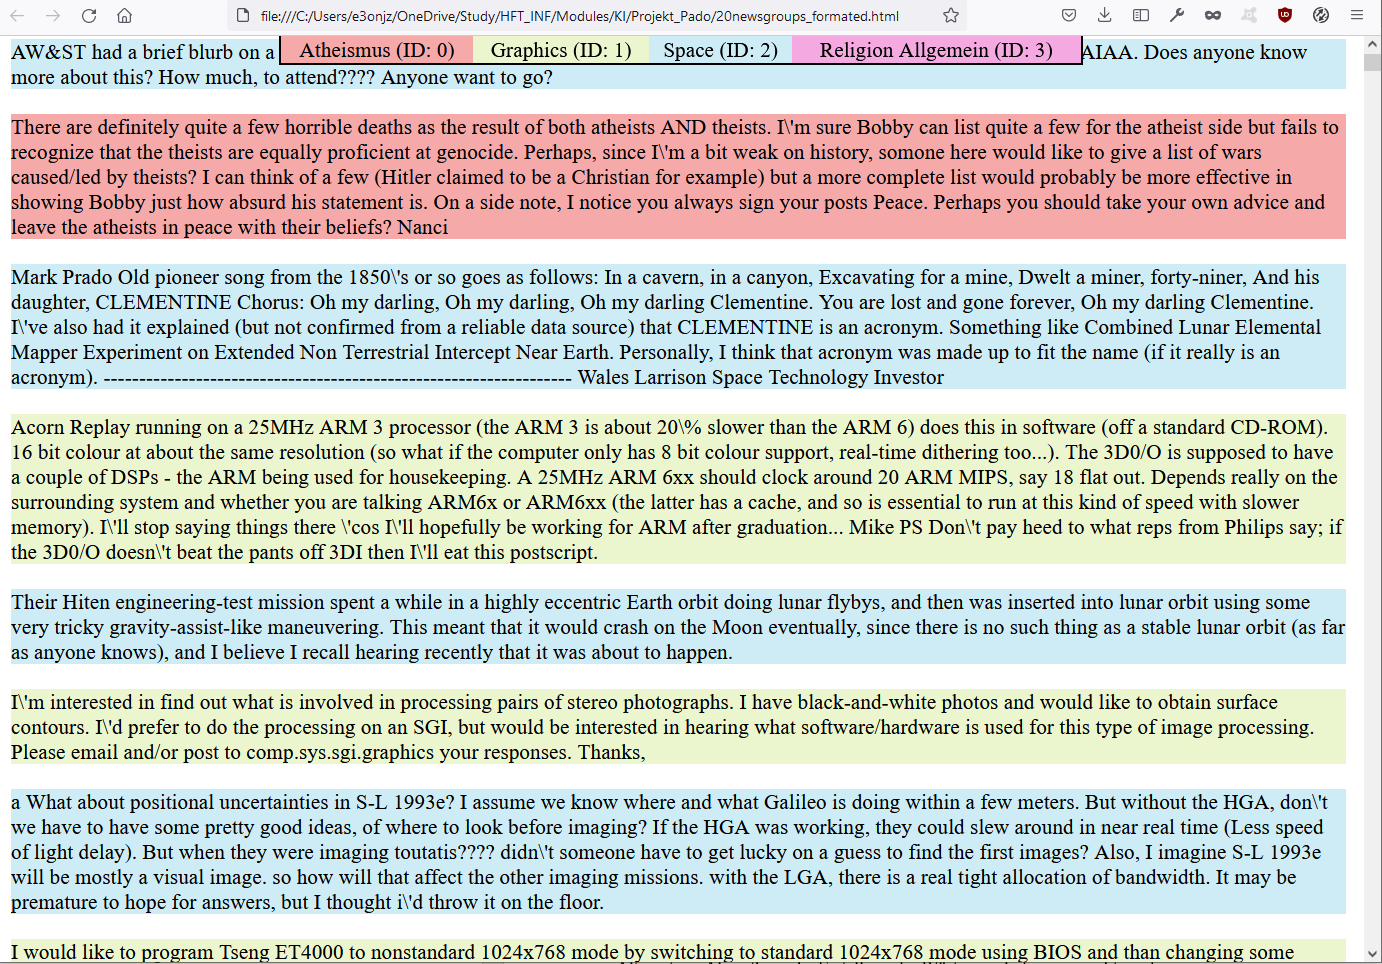
\includegraphics[width=\textwidth]{figures/texte_grafisch_getrennt.png}
	\caption{Texte grafisch nach Kategorie hervorgehoben}
	\label{fig:texte_grafisch_getrennt}
\end{figure}

\begin{figure}[H]
	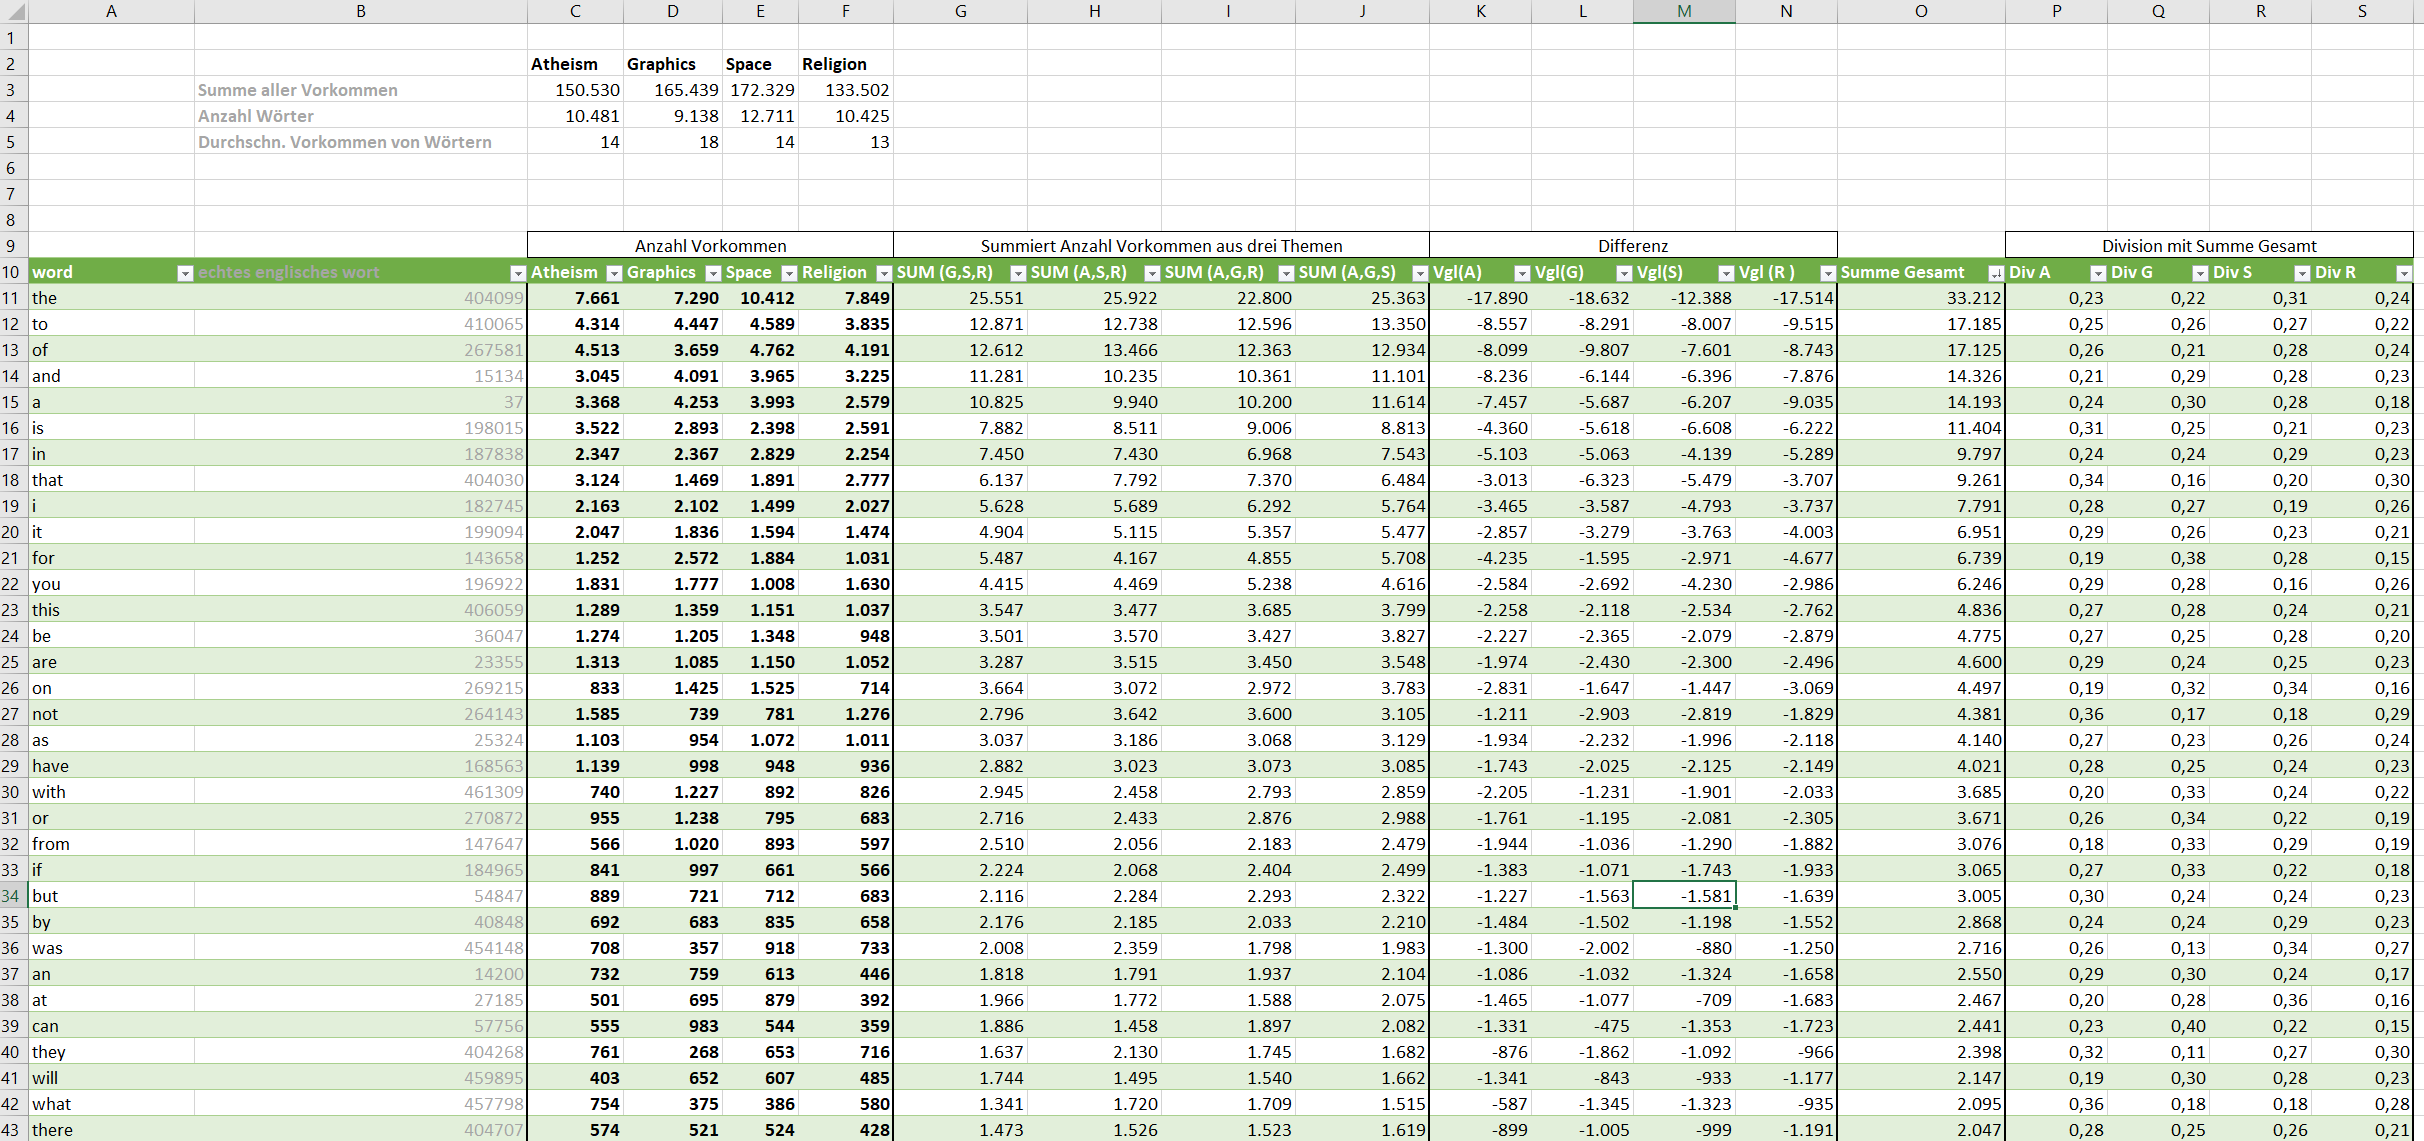
\includegraphics[width=\textwidth]{figures/wort_auswertung_excel.png}
	\caption{Erste Auswertungen über vorkommende Wörter}
	\label{fig:wort_auswertung_excel}
\end{figure}

\begin{figure}[H]
	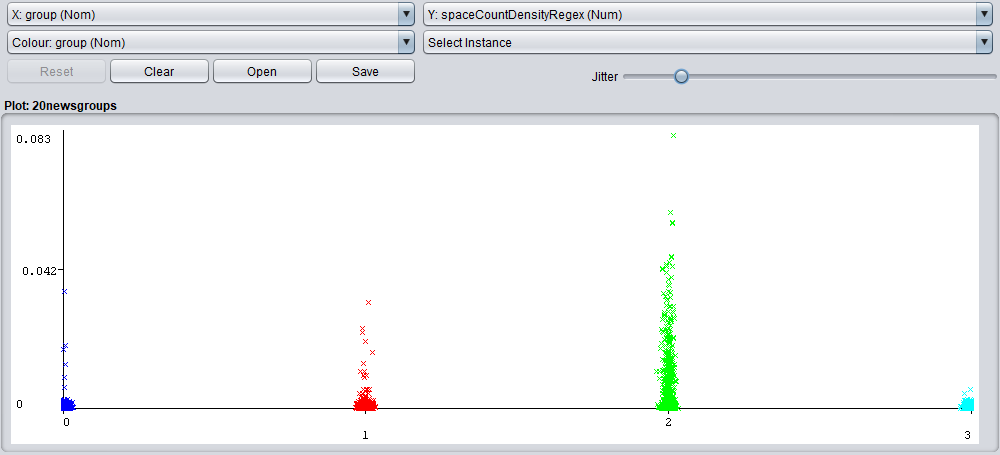
\includegraphics[width=\textwidth]{figures/weka_visualize_space.png}
	\caption{Visualisierung des Features Vorkommen des Wortes \emph{Space}}
	\label{fig:weka_visualize_space}
\end{figure}

\begin{figure}[H]
	\center
	\begin{tabular}{l||c|c|c}
		\textbf{Zielklasse} & \textbf{Precision} & \textbf{Recal} & \textbf{F-Wert} \\ 
		\hline
		\hline
		\textbf{0 (Atheismus)} 		& 0,686 & 0,628 & 0,656 \\ 
		\textbf{1 (Computergrafik)} & 0,724 & 0,835 & 0,776 \\ 
		\textbf{2 (Raumfahrt)} 		& 0,745 & 0,716 & 0,730 \\ 
		\textbf{3 (Religion)} 		& 0,521 & 0,500 & 0,510 \\ 
		\hline
		\textit{Durchschnitt} 		& 0,690 & 0,691 & \textbf{0,689} \\ 
	\end{tabular} 
	\caption{Detailierte Genauigkeit pro Klasse}
	\label{fig:detailed_accuracy_by_class}
\end{figure}

\begin{figure}[H]
	\center
	\begin{tabular}{c|c|c|c||l}
	\textbf{a} & \textbf{b} & \textbf{c} & \textbf{d} & $\leftarrow$ Klassifiziert als \\ 
	\hline 
	\hline 
	\circled{59} 	& 9 	& 10 	& 16 	& \textbf{a} (Atheismus) \\ 
	4 	& \circled{76} 	& 7 	& 4 		& \textbf{b} (Computergrafik) \\ 
	10 	& 16 	& \circled{73} 	& 3 		& \textbf{c} (Raumfahrt) \\ 
	13 	& 4 	& 8 	& \circled{25} 		& \textbf{d} (Religion) \\ 
	\end{tabular} 
	\caption{Verwechslungs Matrix}
	\label{fig:confusion_matrix}
\end{figure}


\end{document}
